% !TEX TS-program = pdflatexmk
\documentclass[11pt]{article}
\usepackage{fullpage}
\usepackage{amssymb, amsmath, amsthm}
\usepackage{graphicx}
\usepackage{mathpazo}
\usepackage{courier}
\usepackage{subcaption}
\usepackage[section]{placeins}
%\renewcommand{\familydefault}{\sfdefault}
\usepackage{multirow}
\newcommand{\argmax}{\operatorname*{arg \ max}}
\newcommand{\argmin}{\operatorname*{arg \ min}}

\linespread{1}

\title{Applications of topological data analysis to single-cell genomics}
\date{\today}
\author{Keshav Motwani}

\begin{document}
\maketitle
\section{Introduction}

In the recent years, single-cell RNA sequencing (scRNA-seq) has become extremely common to uncover cellular diversity and the understand role of specific cells in biological processes by measuring gene expression in each individual cell within a sample. Previously, it was only possible to measure the gene expression for an entire sample, which was the result of summing the gene expression across all the cells in the sample. However, this only provided an understanding of the average behavior of cells within a sample, requiring more complicated experimental protocols for isolating specific cell types. With scRNA-seq, the resulting data for one sample is in the form of a cells by genes matrix, with most experiments profiling tens of thousands of cells and around 30,000 total genes, and the identity of each cell is inferred based on it's gene expression.

In this paper, we want to understand whether it is possible to distinguish between samples pre- and post-treatment with a drug, in order to understand whether changes are induced in gene expression of cells as a result of treatment, and if so, in which specific cell types. As a proof of concept, we use a dataset from Kang et al. 2018 in which peripheral blood mononuclear cells were isolated from 8 patients, and scRNA-seq done was done pre-treatment and post-treatment with Interferon-$\gamma$, a drug known to induce a variety of immune responses.

In essence, we want to understand differences in the distribution of cells in gene expression space that is caused by a treatment, making this application a perfect fit for using topological data analysis, as we can naturally work with each individual cell within each sample as a point in Euclidean space. Additionally, to our knowledge there currently exist no published methods to classify entire scRNA-seq samples other than to simply average gene expression over all cells in the sample, and applying standard classification algorithms on the averaged data, which defeats the purpose of performing scRNA-seq.

\section{Methods}

\subsection{Data preprocessing}
We use a dataset from Kang et al. 2018 in which peripheral blood mononuclear cells were isolated from 8 patients, and scRNA-seq done was done pre-treatment and post-treatment with Interferon-$\gamma$. This dataset is readily available in the \texttt{R} package \texttt{ExperimentHub} under accession ID \texttt{EH2259}. We only consider cells that have been marked as \texttt{singlet} (to remove dead cells and doublets) and have a cell type that is not \texttt{NA}. Additionally, since the raw data has approximately $30,000$ genes, in order to reduce computation times in computing pairwise distances between cells, we represent each sample based on it's top 50 principal components, and use this in downstream tasks.

\subsection{Simplical complex construction}
For each scRNA-seq sample, we construct a Vietoris-Rips complex with a filtration based on Euclidean distance on the principal component space described in the last section. We choose 200 values of radius equally spaced from $0$ to $R$, where $R$ is chosen to be the $0.1$ quantile of the values inside the pairwise distance matrices. This was a somewhat arbitrary cutoff, but worked well in practice to limit computation time yet provide meaningful results.

\subsection{Persistent homology computations}
From the last section, for each sample $A$, we have a filtered simplicial complex of the form
$$
{\rm VR}_1(A) \subset {\rm VR}_2(A)	 \subset \cdots \subset {\rm VR}_{200}(A).
$$
From this, we can compute the homology in degree $p \in \lbrace 0, 1 \rbrace$, $H_p$, of each of these, where
$$
H_p({\rm VR}_j(A)) = Z_p({\rm VR}_j(A))/B_p({\rm VR}_j(A))
$$ 
where $Z_p$ are the $p$-cycles in ${\rm VR}(A^{(j)})$ and $B_p$ are the $p$-boundaries in ${\rm VR}(A^{(j)})$. The consecutive homology vector spaces are connected by linear maps, resulting in a persistence module of the form 
$$
H_p({\rm VR}_1(A)) \to H_p({\rm VR}_2(A)) \to \cdots \to H_p({\rm VR}_{200}(A)).
$$
Using the structure theorem for persistent homology and the persistence algorithm, we can represent this persistence module (up to isomorphism) by a collection of intervals called a barcode. From these barcodes, for homology in degree 1, we compute their persistence landscapes for downstream statistics and machine learning.

\subsection{Paired sample permutation test}

Let $X_i \sim F({\rm PL}(X_i))$ and $Y_i \sim F({\rm PL}(Y_i))$ denote the pre- and post-treatment sample from the $i$th patient respectively with $F$ denoting a family of distributions indexed by the true persistence landscapes where ${\rm PL}(\cdot)$ is the true persistence landscape vector. We want to test the null hypothesis that the parameters of $F$ are the same pre- and post-treatment, i.e. that ${\rm PL}(X_i) = {\rm PL}(Y_i)$. However, we do not know the true persistence landscapes ${\rm PL}(X_i)$ and ${\rm PL}(Y_i)$, so we use a permutation test based on multiple observed samples pre- and post-treatment and their estimated persistence landscapes $\hat{{\rm PL}}(X_i)$ and $\hat{{\rm PL}}(Y_i)$. We use a test statistic given by
$$
T(X, Y) = ||\frac{1}{N}\sum_{i = 1}^{N} \hat{{\rm PL}}(X_i) -  \hat{{\rm PL}}(Y_i) ||_2.
$$
This turns out to be the same as the test statistic for the two sample permutation test, but here the difference is in the null distribution. Under the null hypothesis, the underlying distribution of $X_i$ and $Y_i$ are the same, and thus we construct permutations that permute treatment status only within the same patient. Let $X^*, Y^*$ denote a permutation where
$$
X^*_i = X_i~\text{or}~Y_i, \quad
Y^*_i =   \begin{cases}
               	X_i & \text{if $X^*_i = Y_i$} \\
                  Y_i & \text{otherwise} \\
 			 \end{cases}.
$$
There are $2^N$ such permutations, so we enumerate through these and compute $T(X^*, Y^*)$ for each to construct the null distribution.

\section{Results}

\subsection{Analysis of global effects}
We first analyzed the effects of treatment on all cell types combined by computing the Vietoris-Rips complex for each sample. From this we computed the persistence diagram, and finally the persistence landscape for statistical comparisons. The persistence diagrams of homology in degree 0 and degree 1 are shown in Figure 1(a), and the barcodes of homology in degree 1 are shown in Figure 1(b). These show at what time/radius a particular cycle was born and at what time it becomes a boundary (dies). 

\begin{figure*}[!htb]
    \centering
    \begin{subfigure}[t]{0.5\textwidth}
        \centering
	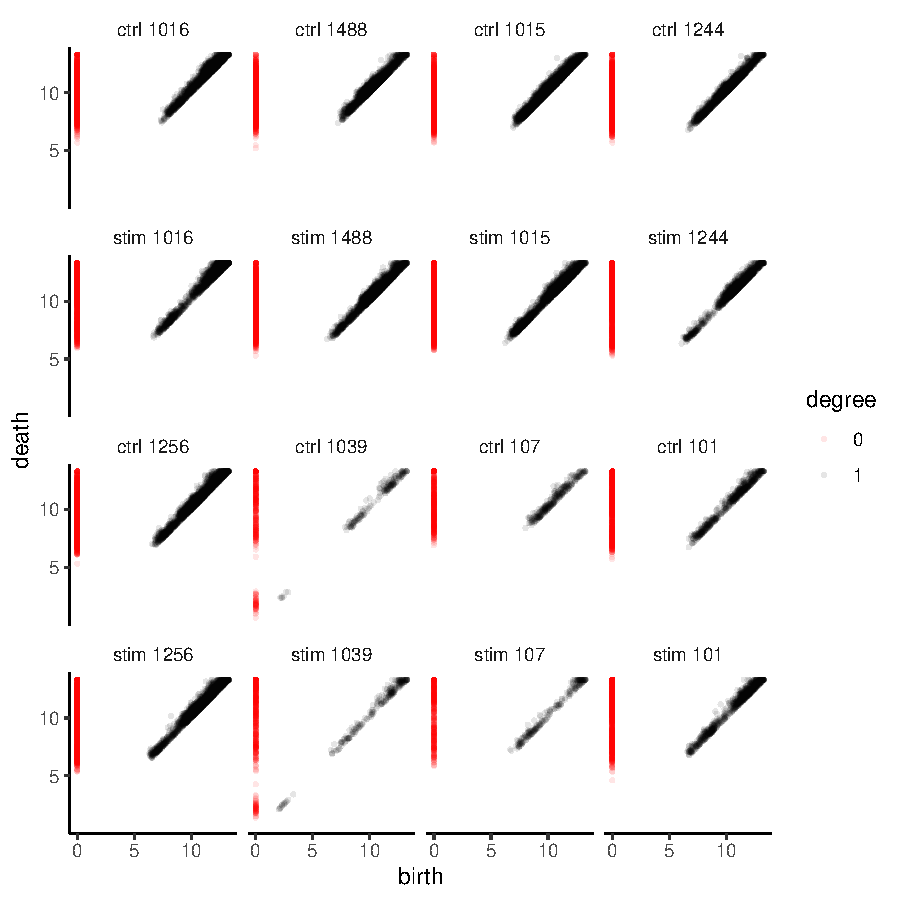
\includegraphics[width=7cm]{results/all_persistence_diagrams.pdf}
        \caption{}
    \end{subfigure}%
    ~ 
    \begin{subfigure}[t]{0.5\textwidth}
        \centering
	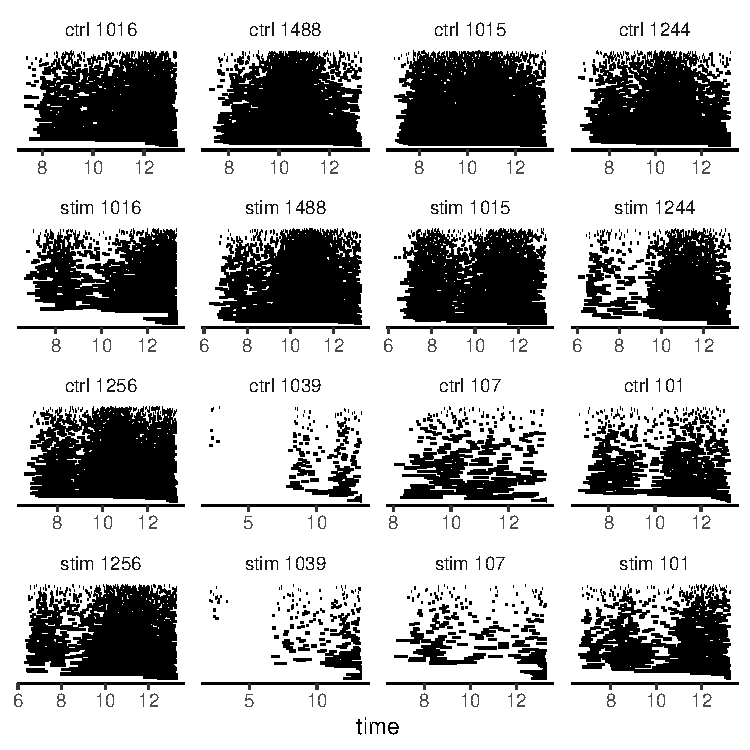
\includegraphics[width=7cm]{results/all_barcodes.pdf}
        \caption{}
    \end{subfigure}
    \caption{Visualization of persistent homology features in all samples. (a) Persistence diagrams showing birth time versus death time for homology in degree 0 (red) and degree 1 (black). (b) Persistence barcodes of homology in degree 1, with each line indicating when a feature was born and dies. Titles at the top of each subplot are labeled with treatment status and patient ID, where ``ctrl" means pre-treatment and ``stim" means post-treatment.}
\end{figure*}

While it is hard to discern clear differences caused by treatment in the persistence diagram plots, converting the persistence diagrams into persistence landscapes shows a clearer picture. The persistence landscapes for each sample are shown in Figure 2. and the difference of average persistence landscapes per treatment status are shown Figure 3. From the difference of average landscapes, we can see that at earlier timepoints, features persist longer post-treatment, at timepoints in the middle, features persist longer pre-treatment, and at later timepoints, features persist longer post-treatment. These differences could possibly be related to specific cell subpopulations, which we explore in more detail in the next section.

\begin{figure*}[!htb]
    \centering
	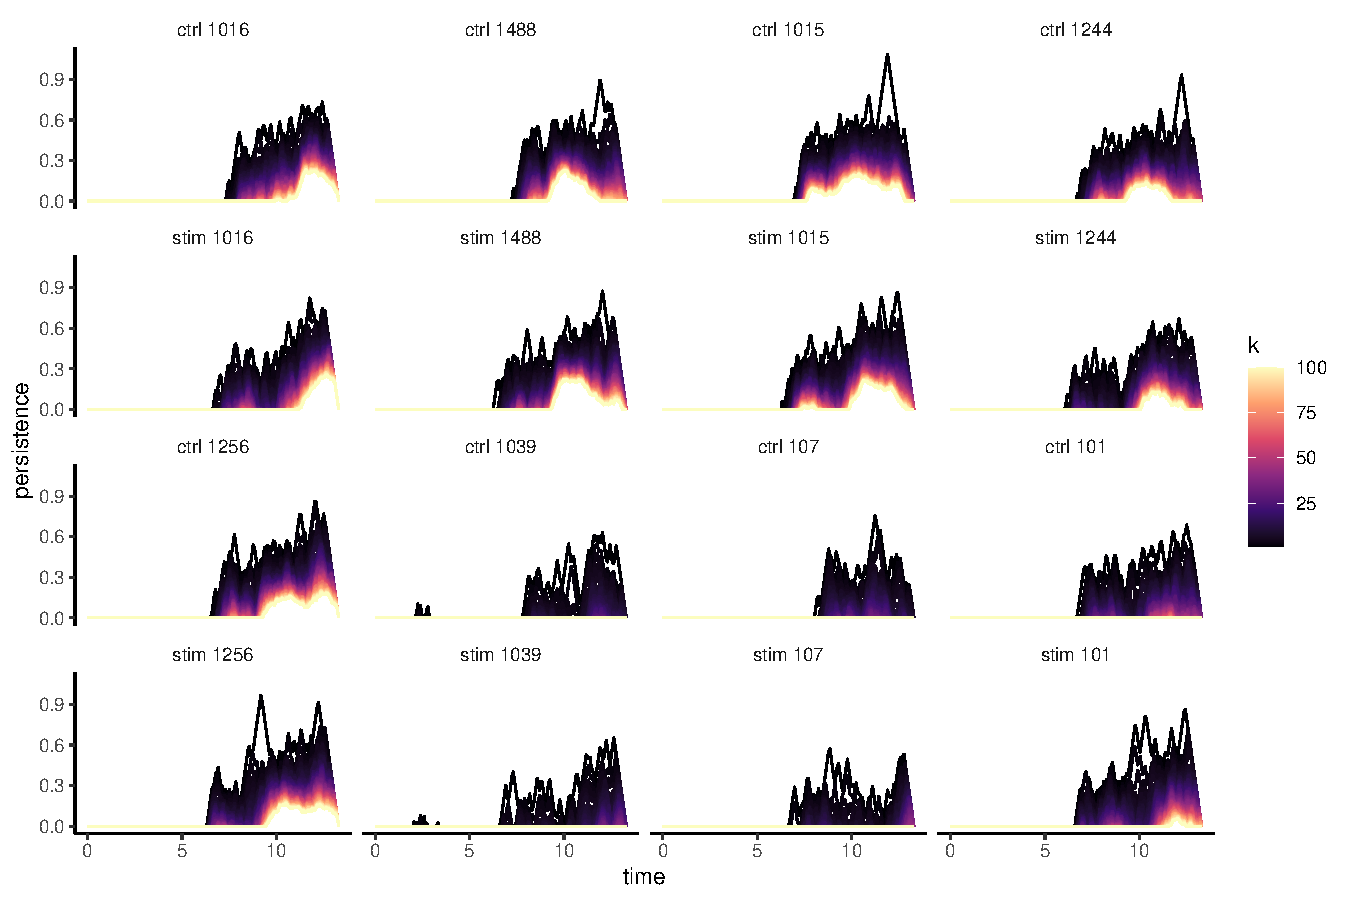
\includegraphics[width=14cm]{results/all_persistence_landscapes.pdf}
    \caption{Result of persistence landscape computation for all samples. Each landscape function is colored as shown in the legend. Titles of each subplot are as in the previous figure.}
\end{figure*}

\begin{figure*}[!htb]
    \centering
	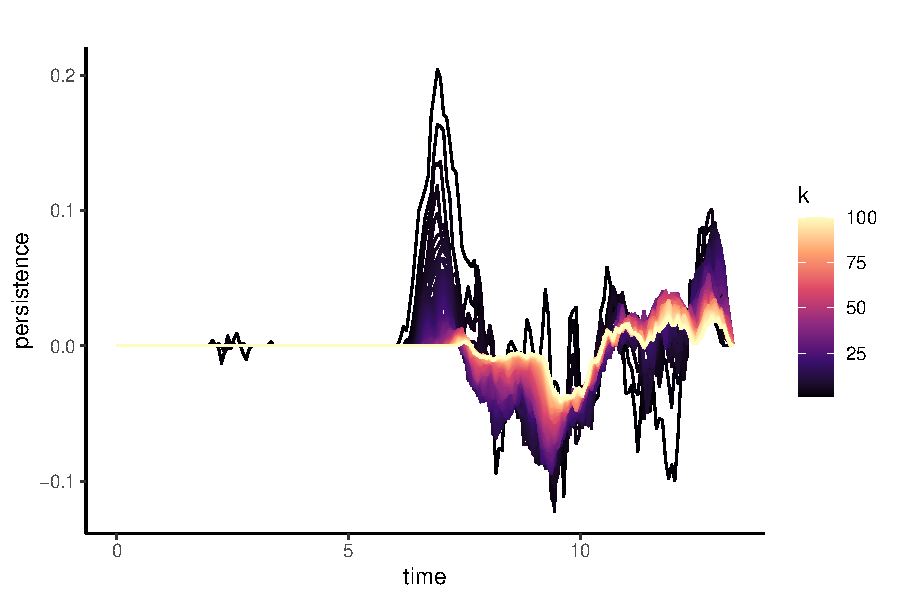
\includegraphics[width=10cm]{results/all_persistence_landscape_difference.pdf}
    \caption{Difference of average persistence landscapes per treatment group. Positive values indicate longer persistence post-treatment, and negative values indicate longer persistence pre-treatment.}
\end{figure*}

To better visualize sources of variability across samples, we perform principal components analysis on the matrix of persistence landscapes, and the first two components are shown in Figure 4. We see that samples cluster mainly by the patient from which it is from, as opposed to treatment status, but we do see that for the most part, post-treatment samples have lower PC2 values compared to their pre-treatment sample, indicating a consistent difference in persistence landscapes caused by treatment.

\begin{figure*}[!htb]
    \centering
	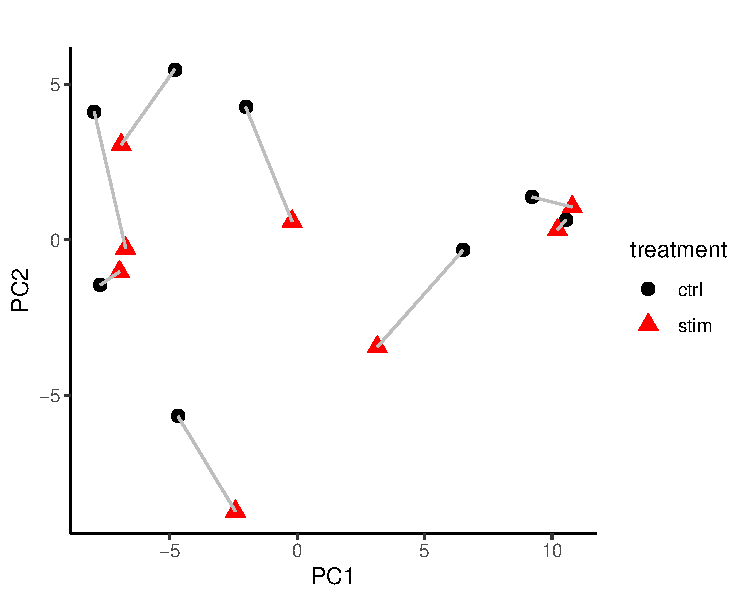
\includegraphics[width=8cm]{results/all_persistence_landscape_pca.pdf}
    \caption{Plot of first two principal components of persistence landscape matrix. Points are colored by treatment status, where ``ctrl" indicates pre-treatment and ``stim" indicates post-treatment. Gray lines connect the samples from the same patient.}
\end{figure*}

To formally test whether the differences between pre- and post-treatment samples are not just due to sampling variability, we perform permutation tests as described in the Methods. In Figure 5, we show the null distribution and observed test statistic for the paired test versus two-sample test. Note that the question of interest is answered by the paired test, that there is a significant difference in persistence landscapes pre- and post-treatment in the same patient, but we also show the results of the two-sample test to highlight the importance of performing a paired test for the particular question of interest.

\begin{figure*}[!htb]
    \centering
	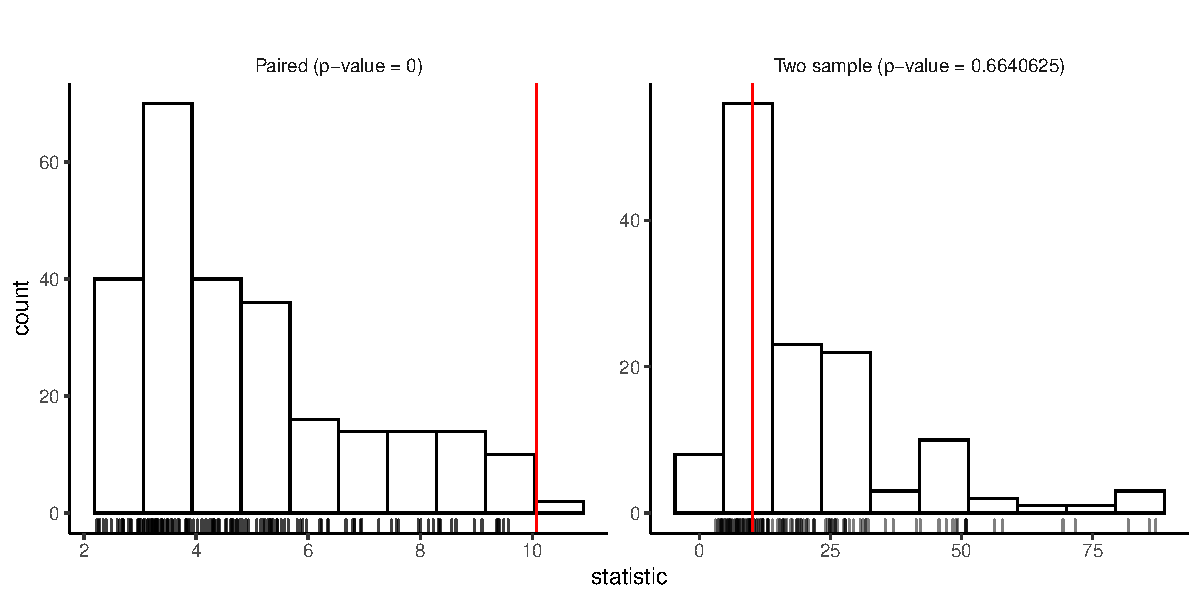
\includegraphics[width=15cm]{results/all_permutation_test.pdf}
    \caption{Permutation test results for paired sample test (left) and two sample test (right). A histogram of the null permutation distribution is shown in black, with individual null test statistics shown as black lines at the bottom. The observed test statistic is indicated with the red line. Titles of subplots include p-value.}
\end{figure*}

\subsection{Analysis of cell type specific effects}

In the previous section, we analyzed the "shape" of all cells in gene expression space. To improve interpretability of the results, we now perform a similar analysis, but on specific subpopulations of cells at a time. To do this, we subset each sample to one of 6 cell types, B cells, CD4+ T cells, FCGR3A+ Monocytes, CD14+ Monocytes, CD8+ T cells, and NK cells. On these subsets, we perform the same persistent homology computations as the last section, and analyze the resulting persistence landscapes. In Figure 6, we show the difference of average persistence landscapes across treatment, per cell type. As hypothesized in the last section, the differences in persistence patterns are largely cell type specific. In some cell types, all features persist longer pre-treatment, while in other cell types, all features persist longer post-treatment, and in cell types with the largest differences due to treatment (CD4+ T cells and CD14+ Monocytes), there is a mixture of the two.

\begin{figure*}[!htb]
    \centering
	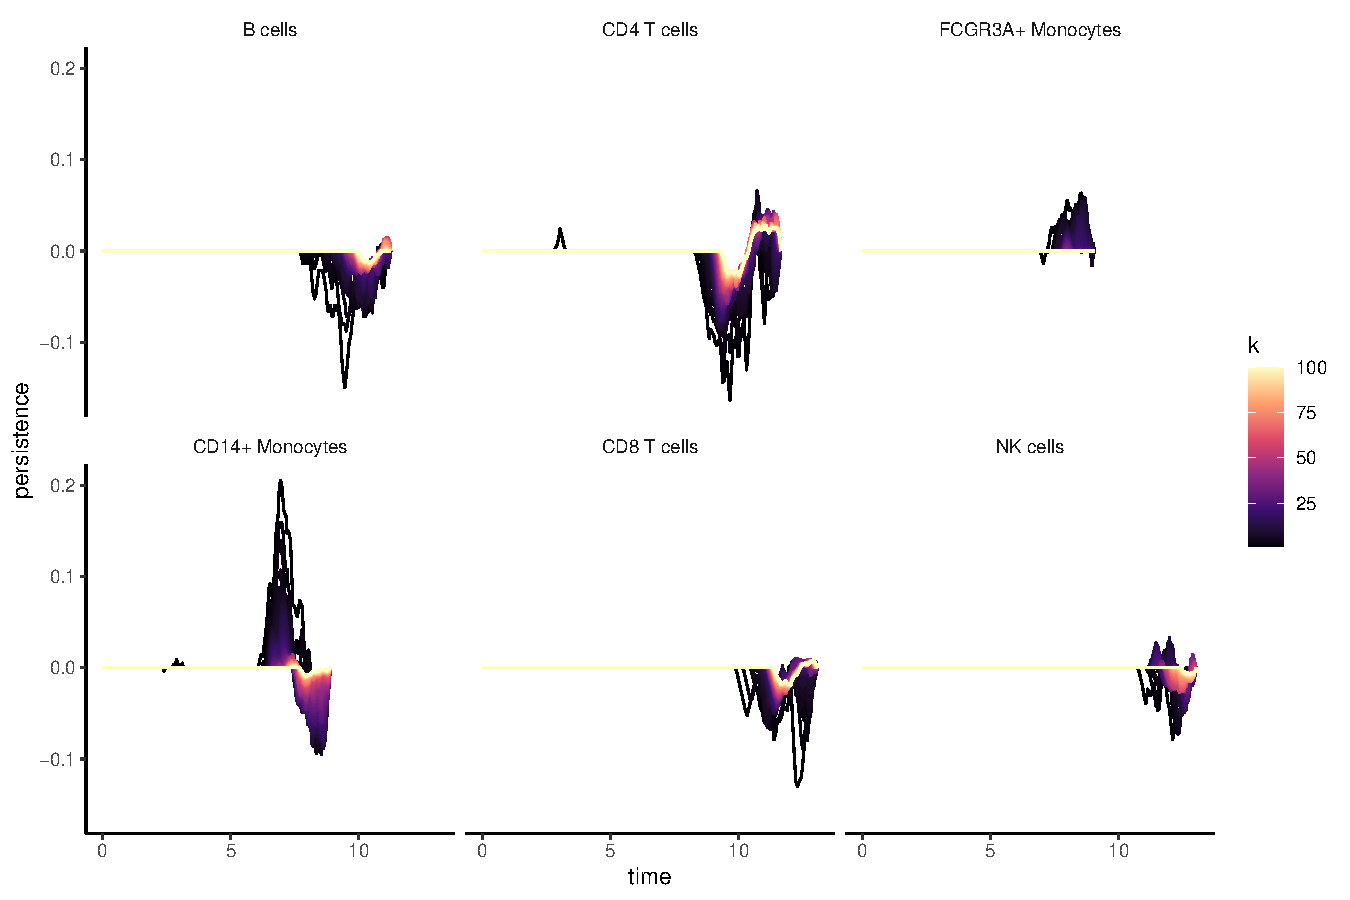
\includegraphics[width=14cm]{results/combined_persistence_landscape_difference.pdf}
    \caption{Difference of average persistence landscapes per treatment group for each cell type separately. Positive values indicate longer persistence post-treatment, and negative values indicate longer persistence pre-treatment. Titles of subplots indicate cell type identity.}
\end{figure*}

Once again, we performed principal components analysis to visualize sources of variation in the data, and the first two components are shown in Figure 7. For all cell types other than CD14+ Monocytes, samples once again cluster by patient, however, in CD14+ Monocytes, there is almost clear separation of samples by treatment status. This indicates the treatment effect is larger than the inter-patient variability. CD4+ T cells also indicate some differences pre- and post-treatment, with post-treatment samples generally having higher PC2 values than the corresponding pre-treatment sample.

\begin{figure*}[!htb]
    \centering
	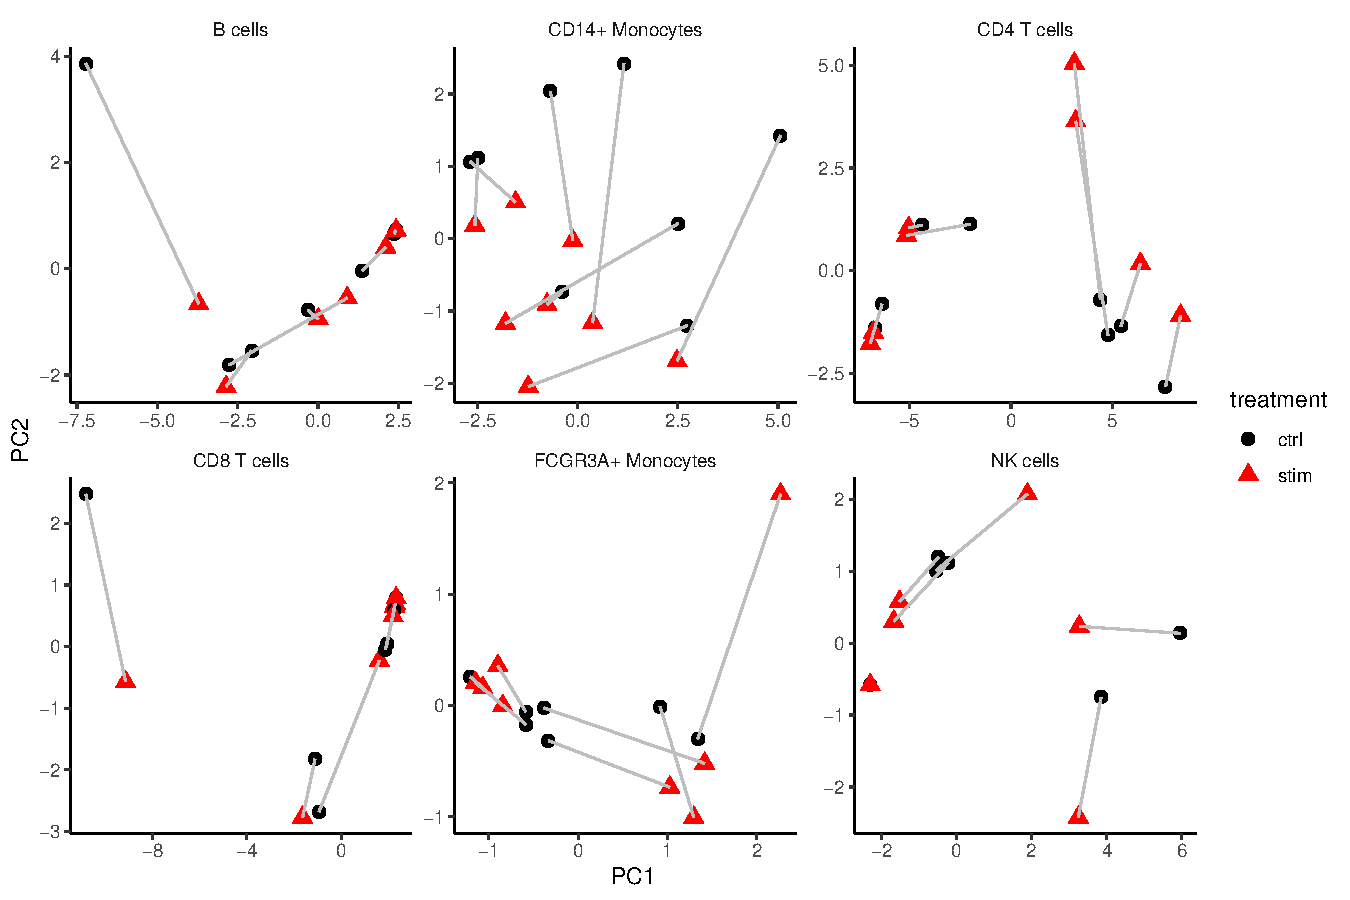
\includegraphics[width=14cm]{results/combined_persistence_landscape_pca.pdf}
    \caption{Plot of first two principal components of persistence landscape matrix for each cell type separately. Points are colored by treatment status, where ``ctrl" indicates pre-treatment and ``stim" indicates post-treatment. Gray lines connect the samples from the same patient. Titles of subplots indicate cell type identity.}
\end{figure*}

Finally, we perform the permutation tests per cell type to formally test whether there was a difference in persistence landscapes pre- and post-treatment. These results are shown in Figure 8. Results from the paired sample permutation test show that only CD14+ Monocytes and CD4+ T cells had significant p-values. 

\begin{figure*}[!htb]
    \centering
	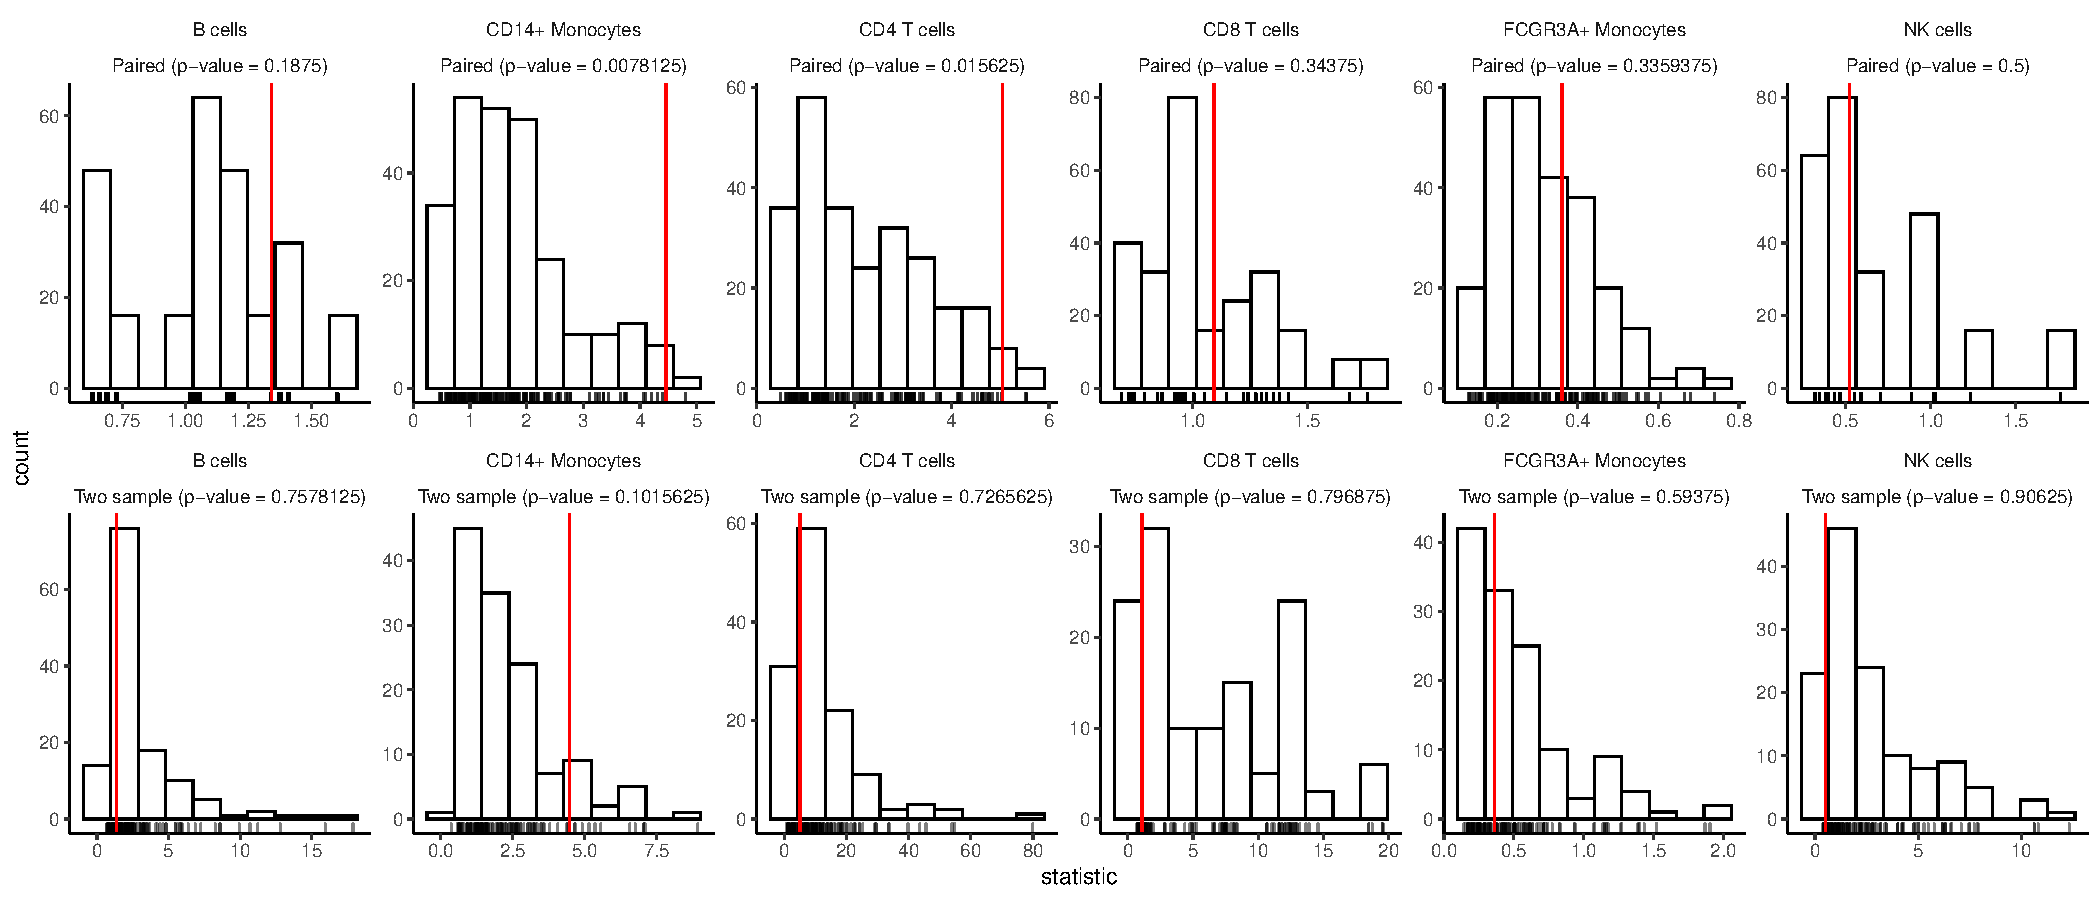
\includegraphics[width=16cm]{results/combined_permutation_test.pdf}
    \caption{Permutation test results for paired sample test (top row) and two sample test (bottom row) for each cell type separately (columns). A histogram of the null permutation distribution is shown in black, with individual null test statistics shown as black lines at the bottom. The observed test statistic is indicated with the red line. Titles of subplots include p-value and also indicate cell type identity.}
\end{figure*}

\section{Conclusion}

In this project we showed that topological data analysis, specifically using persistence landscapes, is able to encode the differences caused by treatment and yield biological insight. We found that CD14+ Monocytes and CD4+ T cells had the largest change due to treatment with Interferon-$\gamma$. While the use-case in this example was just a proof-of-concept with a relatively simple treatment and only few samples, this method has promise for more meaningful applications, specifically in mechanistic analyses of clinical trials. For treatments that have larger treatment effects, there is a possibility of using this method for classification of samples, for example to classify responders versus non-responders of a particular drug, to help enable personalized medicine in the future. 

\end{document}
